\subsection{UC7 – Ricerca di un locale tramite nome}
\begin{center}
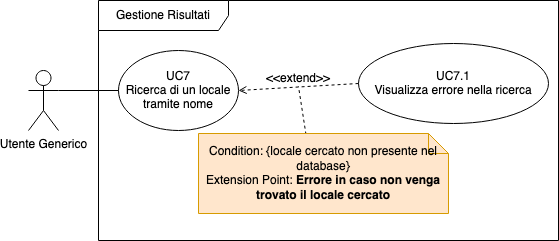
\includegraphics[scale=0.5]{UC_images/UC7.png} 
\end{center}
\begin{itemize}
    \item \textbf{Attore primario}: Utente generico.
    \item \textbf{Precondizione}: L'utente si trova all’interno della piattaforma Sweeat.
    \item \textbf{Postcondizione}: Viene visualizzato la lista dei locali ricercati.
    \item \textbf{Scenario principale}: 
    \begin{enumerate}
        \item L’utente va nella barra di ricerca della piattaforma;
        \item L’utente digita il nome del locale da cercare;
        \item L’utente clicca sul bottone di ricerca;
    \end{enumerate}
    \item \textbf{Estensioni}:
    \begin{itemize}
        \item Nel caso in cui l’utente l’utente inserisce il nome di un locale inesistente
	\begin{enumerate}  
		\item L’utente va nella barra di ricerca della piattaforma;
        \item L’utente digita il nome del locale da cercare;
        \item L’utente clicca sul bottone di ricerca; 
        \item Viene mostrato un messaggio d'errore, nel caso non sia presente alcun locale (UC7.1 §).
    	%Visualizzazione di un messaggio informando che non è presente nessun locale con tale nome e viene suggerita una lista di locali simili a quello ricercato.   
    \end{enumerate}
    \end{itemize}    
\end{itemize}

\subsubsection{UC7.1 – Visualizza errore nella ricerca}
\begin{itemize}
\item \textbf{Attore primario}: Utente Generico.
\item \textbf{Precondizione}: L'utente si trova all’interno della piattaforma Sweeat.
\item \textbf{Postcondizione}: Viene mostrato un messaggio d'errore e l'utente non è in grado di visualizzare il locale cercato.

\item \textbf{Scenario principale}:
\begin{enumerate}
	\item L'operazione di ricerca del locale desiderato fallisce;
	\item Viene mostrato il corrispondente messaggio d'errore;
	\item All'utente viene data la possibilità di visualizzare dei locali alternativi di cercare nuovamente il locale desiderato.
\end{enumerate}
\end{itemize}